\section{Further empirical investigation of Goodharting}\label{appendix: results}

\subsection{Additional plots for the Goodharting prevalence experiment}

\begin{figure}[htbp]
    \centering
    \begin{subfigure}[tb]{0.45\textwidth}
        \centering
        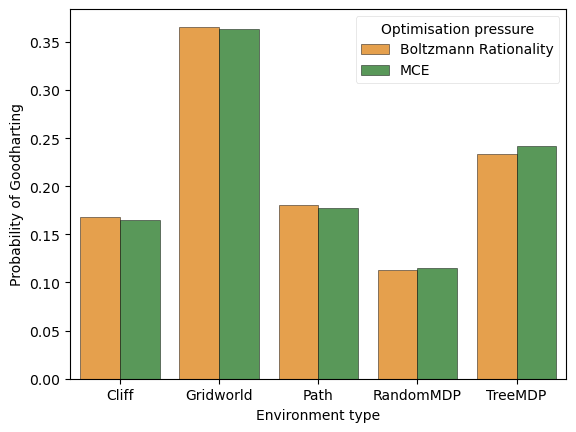
\includegraphics[width=0.9\textwidth]{metrics/type-prob-goodharting.png}
        \caption{The relationship between the type of environment and the probability of Goodharting.\label{fig:type-prob-goodharting}}
    \end{subfigure}
    \hfill
    \begin{subfigure}[tb]{0.45\textwidth}
        \centering
        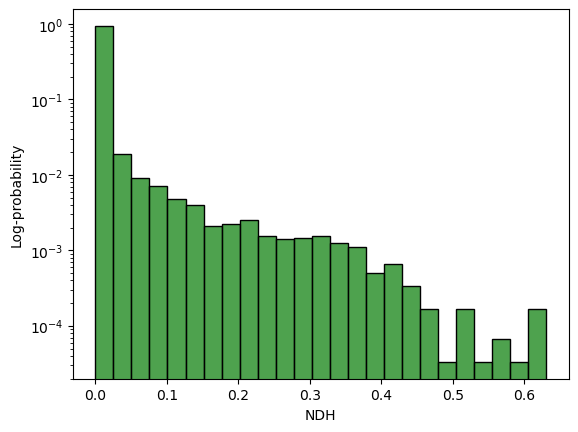
\includegraphics[width=0.9\textwidth]{metrics/distribution-of-ndh.png}
        \caption{Log-scale histogram of the distribution of \textbf{NDH metric} in the dataset.\label{fig:distribution-of-ndh}}
    \end{subfigure}
    \caption{Summary of the experiment described in~\Cref{sec:quantifying_goodharting}. (a) The choice of operationalisation of optimisation pressure does not seem to change results in any significant way. (b) NDH metric follows roughly exponential distribution when restricted to cases when NDH > 0.}
\end{figure}


\subsection{Examining the impact of key environment parameters on Goodharting}
To further understand the conditions that produce Goodharting, we investigate the correlations between key parameters of the MDP, such as the number of states or temporal discount factor $\gamma$, and NDH. Doing it directly over the dataset described in~\Cref{sec:quantifying_goodharting} does not yield good results, as there is not enough data points for each dimension, and there are confounding cross-correlations between different parameters changing at the same time.

To address those issues, we opted to replace the grid-search method that produced the datasets for~\Cref{sec:quantifying_goodharting} and ~\Cref{sec:evaluation}. We have first picked a base distribution over representative environments, and then created a separate dataset for each of the key parameters, where only that parameter is varied.\footnote{Since this is impossible when comparing between environment types, we use the original dataset from~\Cref{sec:quantifying_goodharting} in~\Cref{fig:ndh-type}.}

Specifically, the base distributions is given over \emph{RandomMDP} with $|S|$ sampled uniformly between $8$ and $64$, $|A|$ sampled uniformly between $2$ and $16$, and the number of terminal states sampled uniformly between $1$ and $4$, where $\gamma = 0.9$, $\sigma = 1$, and where we use 25 $\lambda$'s spaced equally (on a log scale) between $0.01$ and $0.99$. Then, in each of the runs we modify this base distribution of environments along a single axis, such as sampling $\gamma$ uniformly across $(0, 1)$ shown in~\Cref{fig:ndh-gamma}.

\paragraph{Key findings (positive):} The number of actions $|A|$ seems to have a suprisingly significant impact on NDH (\Cref{fig:ndh-a}). The further away is the proxy reward function from the true reward, the more Goodharting is observed (\Cref{fig:ndh-distance}), which corroborates the explanation given at the end of~\Cref{sec:explain_goodhart}. We note that in many examples (for example in~\Cref{fig:cherrypicked} or in any of graphs in~\Cref{fig:evaluation-all-one}) the closer the proxy reward is, the later the Goodhart "hump" appeared - this positive correlation is presented in~\Cref{fig:hump-distance}. We also find that Goodharting is less significant in the case of myopic agents, that is, there is a positive correlation between $\gamma$ and NDH (\Cref{fig:ndh-gamma}). Type of environment seems to have impact on observed NDH, but note that this might be a spurious correlation.

\paragraph{Key findings (negative):} The number of states $|S|$ does not seem to significantly impact the amount of Goodharting, as measured by NDH (\Cref{fig:ndh-s-small,fig:ndh-s-large}). This suggests that having proper methods of addressing Goodhart's law is important as we scale to more realistic scenarios, and also partially explains the existence of the wide variety of literature on reward gaming (see~\Cref{sec:related-work}). The determinism of the environment (as measured by the Shannon entropy of the transition matrix $\tau$) does not seem to play any role.

\begin{figure}[htbp]
    \centering
    \begin{subfigure}[tb]{0.4\textwidth}
        \centering
        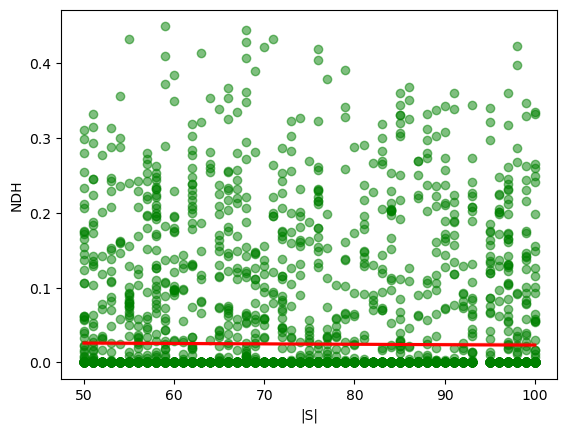
\includegraphics[width=0.9\textwidth]{metrics/sizesmall_ndh.png}
    \end{subfigure}
    \hfill
    \begin{subfigure}[tb]{0.4\textwidth}
        \centering
        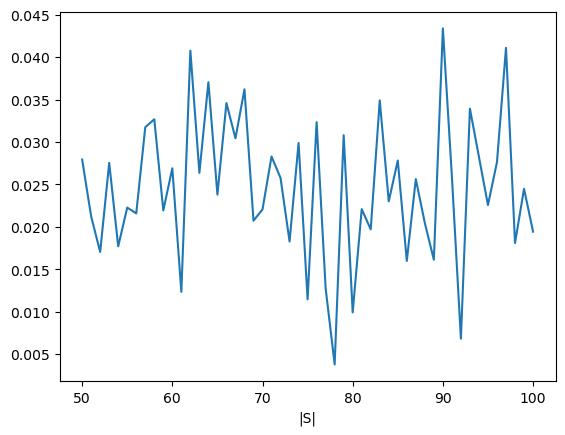
\includegraphics[width=0.9\textwidth]{metrics/sizesmall_ndh_mean.png}
    \end{subfigure}
    \caption{Small negative correlation (not statistically sifnificant) between |S| and NDH: $y = -5e-05x + 0.02852$, 95\% CI for slope: $[-0.00018, 7.23e-05]$, 95\% CI for intercept: $[0.01892, 0.03813]$, Pearson's $r = -0.0119$, $R^2 = 0.0$, $p = 0.4058$. On the left: scatter plot, with the least-squares regression fitted line shown in red. On the right: mean NDH per |S|, smoothed with rolling average, window size=10. \textbf{Below, we have repeated the experiment for larger |S| to investigate asymptotic behaviour.} N=1000.\label{fig:ndh-s-small}}
\end{figure}

\begin{figure}[htbp]
    \centering
    \begin{subfigure}[tb]{0.4\textwidth}
        \centering
        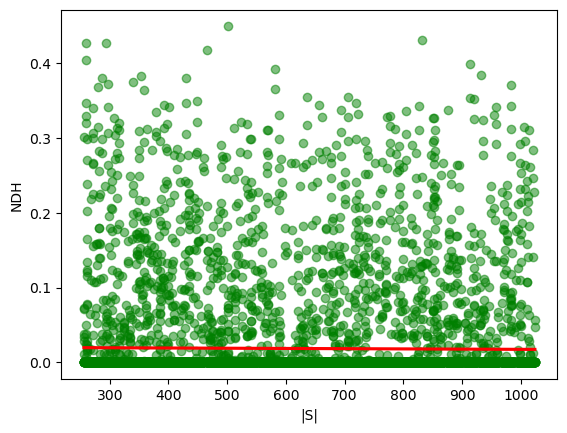
\includegraphics[width=0.9\textwidth]{metrics/size_ndh.png}
    \end{subfigure}
    \hfill
    \begin{subfigure}[tb]{0.4\textwidth}
        \centering
        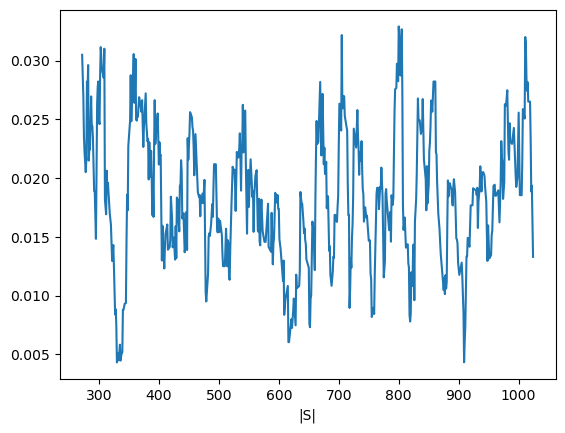
\includegraphics[width=0.9\textwidth]{metrics/size_ndh_mean.png}
    \end{subfigure}
    \caption{Small negative correlation (not statistically significant) between the number of states in the environment and NDH: $y = -0.0x  + 0.02047$, 95\% CI for slope: $[-8.2529e-06, 2.2416e-06]$, 95\% CI for intercept: $[0.017, 0.0239]$, Pearson's $r = -0.0116$, $R^2 = 0.0$, $p = 0.261$. On the left: scatter plot, with the least-squares regression fitted line shown in red. On the right: mean NDH per |S|, smoothed with rolling average, window size=10. N=1000.\label{fig:ndh-s-large}}
\end{figure}

\begin{figure}[htbp]
    \centering
    \begin{subfigure}[tb]{0.4\textwidth}
        \centering
        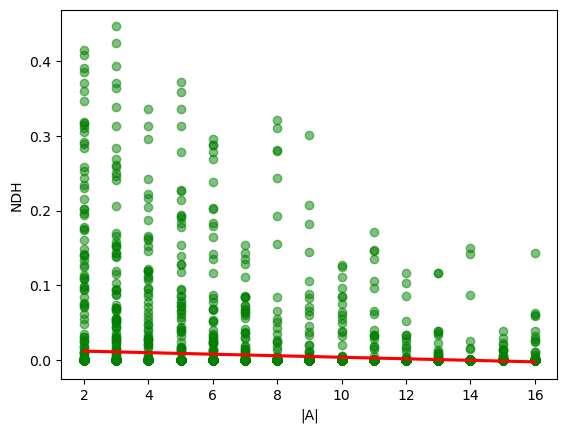
\includegraphics[width=0.9\textwidth]{metrics/actions_ndh.png}
    \end{subfigure}
    \hfill
    \begin{subfigure}[tb]{0.4\textwidth}
        \centering
        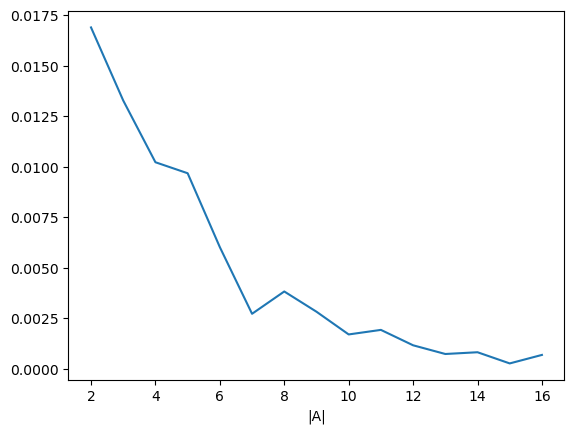
\includegraphics[width=0.9\textwidth]{metrics/actions_ndh_mean.png}
    \end{subfigure}
    \caption{Correlation between |A| and NDH: $y = -0.00011x + 0.00871$, 95\% CI for slope: $[-0.00015, -7.28e-05]$, 95\% CI for intercept: $[0.00723, 0.01019]$, Pearson's $r = -0.0604$, $R^2 = 0.0$, $p < 1e-08$. On the left: scatter plot, with the least-squares regression fitted line shown in red. On the right: mean NDH per |A|. N=1000.\label{fig:ndh-a}}
\end{figure}

\begin{figure}[htbp]
    \centering
    \begin{subfigure}[tb]{0.45\textwidth}
        \centering
        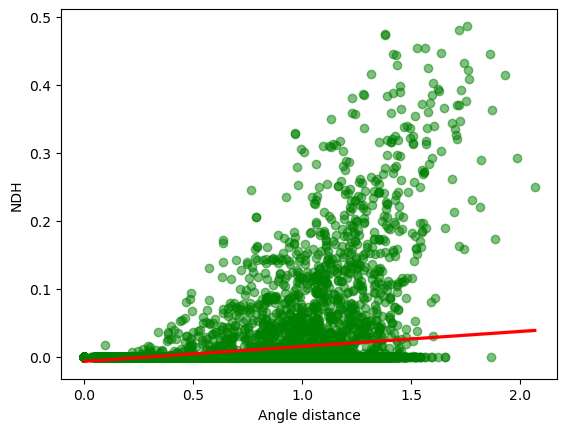
\includegraphics[width=0.9\textwidth]{metrics/distance_ndh.png}
        \caption{Correlation between the angle distance to the proxy reward and \textbf{NDH metric}: $y = 0.02389x - 0.00776$, 95\% CI for slope: $[0.02232, 0.02546]$, 95\% CI for intercept: $[-0.00883, -0.00670]$, Pearson's $r = 0.2895$, $R^2 = 0.08$, $p < 1.2853e-187$.\\\label{fig:ndh-distance}}
        \label{fig: dropvsdims1}
    \end{subfigure}
    \hfill
    \begin{subfigure}[tb]{0.45\textwidth}
        \centering
        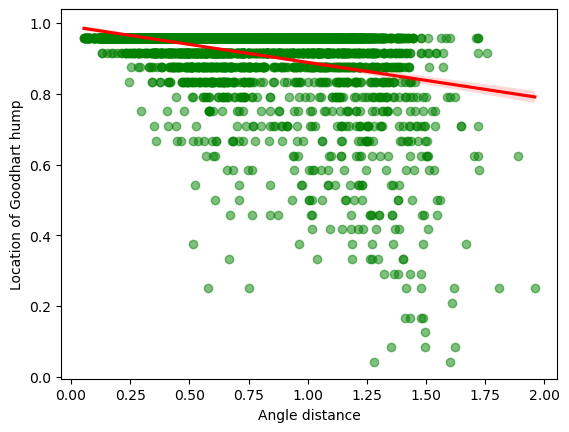
\includegraphics[width=0.9\textwidth]{metrics/goodhart_hump_location.png}
        \caption{Correlation between the distance to the proxy reward, and the \textbf{location of the Goodhart's hump}: $y = -0.10169x + 0.99048$, 95\% CI for slope: $[-0.11005, -0.09334]$, 95\% CI for intercept: $[0.98360, 0.99736]$, Pearson's $r = -0.3422$, $R^2 = 0.12$, $p < 2.7400e-118$.\label{fig:hump-distance}}
    \end{subfigure}
    \hfill
    \begin{subfigure}[tb]{0.45\textwidth}
        \centering
        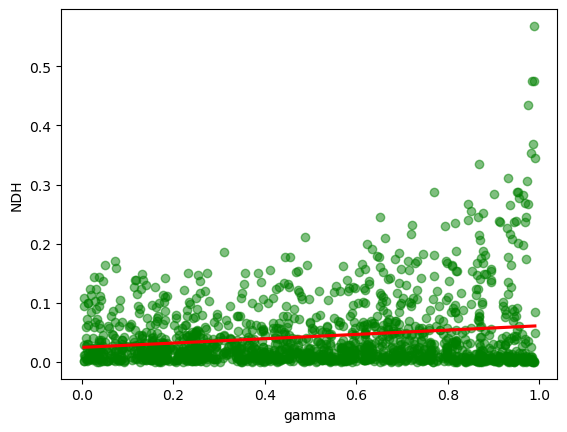
\includegraphics[width=0.9\textwidth]{metrics/gamma_ndh.png}
        \caption{Correlation between $\gamma$ and the \textbf{NDH metric}: $y = 0.00696x + 0.00326$, 95\% CI for slope: $[0.00504, 0.00888]$, 95\% CI for intercept: $[0.00217, 0.00436]$, Pearson's $r = 0.07137$, $R^2 = 0.01$, $p < 1.2581e-12$. \label{fig:ndh-gamma}}
    \end{subfigure}
    \hfill
    \begin{subfigure}[tb]{0.45\textwidth}
        \centering
        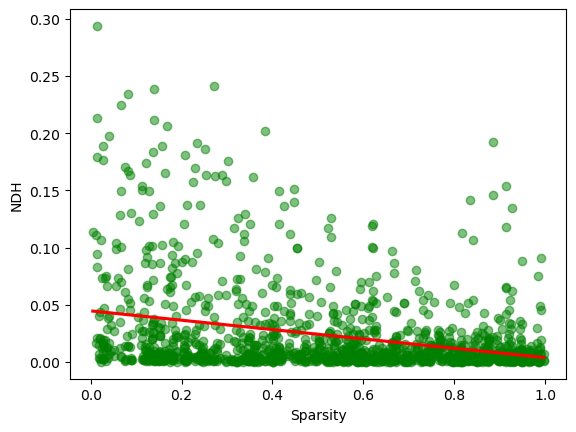
\includegraphics[width=0.9\textwidth]{metrics/sparsity_ndh.png}
        \caption{Correlation between the sparsity of the reward, and the \textbf{NDH metric}: $y = -0.00701x + 0.00937$, 95\% CI for slope: $[-0.00852, -0.00550]$, 95\% CI for intercept: $[0.00850, 0.01024]$, Pearson's $r = -0.09090$, $R^2 = 0.01$, $p < 9.5146e-20$.\label{fig:ndh-sparsity}}
    \end{subfigure}
    \hfill
    \begin{subfigure}[tb]{0.45\textwidth}
        \centering
        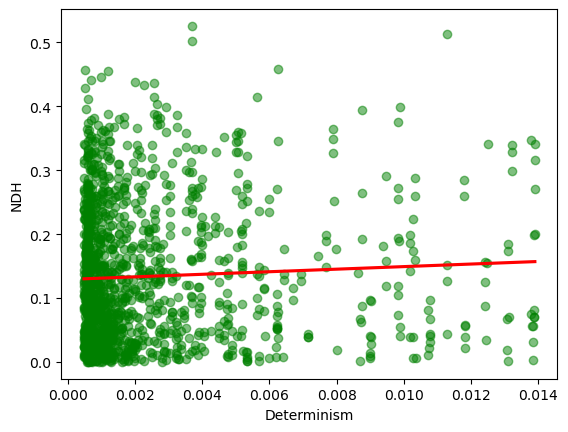
\includegraphics[width=0.9\textwidth]{metrics/determinism_ndh.png}
        \caption{Correlation between the determinism of the environment, and the \textbf{NDH metric}: $y = 0.77221x + 0.01727$, 95\% CI for slope: $[0.31058, 1.23384]$, 95\% CI for intercept: $[0.01570, 0.01884]$, Pearson's $r = 0.03278$, $R^2 = 0.01$, $p = 0.0010$.\label{fig:ndh-determinism}}
    \end{subfigure}
    \hfill
    \begin{subfigure}[tb]{0.45\textwidth}
        \centering
        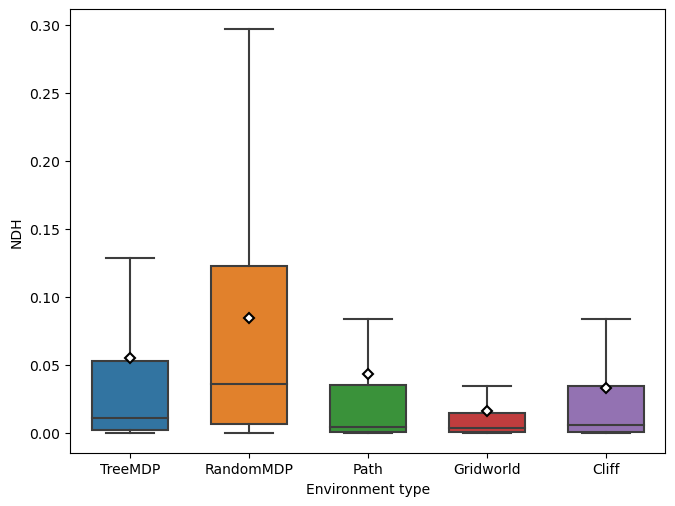
\includegraphics[width=0.9\textwidth]{metrics/ndh-env.png}
        \label{fig: dropvsdims2}
        \caption{Distribution of NDH metric for different kinds of environments. Note that other parameters are \emph{not} kept constant across environments, which might introduce cross-correlations.\\ \\ \label{fig:ndh-type}}
    \end{subfigure}
    \caption{Correlation plots for different parameters of MDPs. N=1000 for all graphs above except for~\Cref{fig:ndh-type}, which uses the dataset from~\Cref{sec:quantifying_goodharting} where N=30400.}
    \label{fig:goodhart-trends-five}
\end{figure}

